In this chapter, the methods used to investigate the problem statement are
presented. First, the choice of method is described briefly and motivated, this
section will also cover the databases used and why these were picked. Following
this section comes a section describing the benchmark problems, that is the
dataset used and the corresponding queries. Finally the implementation details
of the tool used is described in more detail.

\section{Choice of method}\label{sec:choiceofmethod}
This section begins with a short motivation to why the choice of method in
general. Following this is a description of the databases and why these were
chosen. After this is a section on the dataset used, both data and queries
against the data. Finally is a section on the hardware used to test on and a
motivation for the choice of technologies used to implement the tool of evaluation.

\subsection{Motivation of method}
The method of evaluation was chosen for a number of reasons:
\begin{itemize}
\item The dataset used should be based on real-world data to capture the
  complexity of databases;
\item All benchmarks should be done in such a way that they provide consistent
  results;
\item And the method developed should be generic and allow multiple queries and
  databases to be tested with the same methods and algorithms.
\end{itemize}

\subsection{Choice of databases}\label{sec:choiceofdatabases}
The two database chosen to be evaluated are PostgreSQL and MariaDB.
Both of these databases fulfill the following criteria:
\begin{enumerate}
\item Modern databases that see much use and development;
\item Open-source projects with code that anyone can read, modify and help develop;
\item And they implement state-of-the-art algorithms and methods.
\end{enumerate}

In addition to this PostgreSQL is the typical choice for academic evaluation.
All research papers mentioned in Chapter~\ref{chap:relatedwork} that have
implemented new algorithms or modified old ones have done so in PostgreSQL.
MariaDB on the other hand is compatible with MySQL making it a common
alternative for enterprises. The two databases should therefore cover the most
commonly used open-source databases for academia and enterprises.

Studying these two databases should cover how well a modern state-of-the-art
query optimizer performs. In addition, as mentioned in Section~\ref{sec:purpose}
since both of them are open-source, if one performs better than the other the
code can be studied to identify areas of improvement.

\subsection{Choice of dataset}
The dataset used for evaluation is one taken directly from the real-world, this
is to ensure that the database has all the traits of a real database:
non-trivial indexes, non-uniform and skewed data as well as a considerable
amount of data.

\subsubsection{The database}
The database was selected primarily because of the fact that it is a real-world
database, and as such has complex relations, indexes and skewed distributions.
The databases otherwise used most commonly for evaluation are
TPC-H~\cite{tpc_th}, TPC-DS~\cite{tpc_tha} or more recently
JOB~\cite{leis_2015_how_hgaqor}, all of which have trivial index setups with
one index per relation on the primary key only. The problem of selecting the
correct index is therefore not possible to evaluate as the index selection is
trivial.

For a more in-depth look at the statistics of the database used for evaluation
see, Section~\ref{sec:benchmark}.

\subsubsection{The queries}
The queries used for evaluation are all variations of one, complex query. The
reason is that:
\begin{itemize}
\item The tables must be sufficiently large to require the cardinality to be
  estimated via sampling;
\item The indexes on the relation must be sufficiently many such that there are
  more than one possible alternative for query optimizer.
\end{itemize}

These two criteria are not fulfilled for more than a few tables in a database,
but it is typically these that will also require the most time to access.

\subsection{Choice of technologies used}
The technologies used to develop the tool used for evaluation were chosen to be
Clojure~\cite{clojure_c}. The choice was done primarily for two reasons:
\begin{enumerate}
\item It runs on the JVM, making the tool platform independent;
\item And Clojure is a high-level language well suited to transforming data in
  simple ways.
\end{enumerate}

For more information regarding the implementation of the tool, see
Section~\ref{sec:implementation}.

\section{Benchmark problems}\label{sec:benchmark}
This section will give a description if the problems used for benchmarking the
query optimizers. The sections starts with a short description of the hardware
used. Following this is a section covering the relevant statistics of the
dataset used. Finally is a description of the queries used for evaluation.

\subsection{Hardware specs}
The hardware used for testing is a dedicated computer running only the databases
and nothing else. The configuration parameters for the database are those of a
standard setup for PostgreSQL and MariaDB respectively.

The specifications of the hardware are:
\begin{itemize}
\item 2 \textit{Intel® Xeon® Processor E5-2643 (10M Cache, 3.30 GHz, 8.00 GT/s Intel®
    QPI)}, featuring 4 cores each;
\item 1 \textit{Seagate Savvio 15K.3 ST9146853SS 146GB 15000 RPM 64MB Cache SAS 6Gb/s
    2.5"}, used to store the project itself on;
\item 1 \textit{Seagate Constellation ES.3 ST4000NM0023 4TB 7200 RPM 128MB Cache SAS
    6Gb/s 3.5"}, used to store the PostgreSQL database on;
\item And 1 \textit{Seagate Constellation ES ST2000NM0001 2TB 7200 RPM 64MB Cache SAS 6Gb/s
    3.5"}, used to store the MariaDB database on.
\end{itemize}

Although it is worth noting that the hardware should have no, or very little,
effect on the query optimizer's plan selection.

\subsection{The dataset}
The dataset is taken from the real-world and describes the data behind one of
TriOptima's products, TriReduce~\cite{portfolio_pcsfoddt|t}. The more relevant
metrics of the dataset can be seen in Table~\ref{table:dataset}, which shows the
number of indexes, number of rows and the size in bytes for the entire database
and the tables used in the queries.

\begin{table}
  \begin{center}
    \begin{tabu} {c c c c}
      \toprule
      name & \#index & \#rows & size (MB) \\
      \midrule
      database total & 1130 & 305 & 1165290 \\
      mm & 6 & 64882651 & 9448 \\
      book & 6 & 51709 & 10 \\
      resamb & 3 & 40598 & 5 \\
      bti & 3 & 0 & 0.05 \\
      cmm & 2 & 17335822 & 1219 \\
      cmt & 9 & 52808814 & 12811 \\
      t & 35 & 115851469 & 92633 \\
      est & 32 & 33726190 & 19434 \\
      ct & 23 & 115751571 & 72320 \\
      mt & 9 & 21721256 & 4284 \\
      \bottomrule
    \end{tabu}
    \caption[The metrics for the dataset]{The metrics for the dataset used for
      evaluation of the databases. Both the metrics for the entire database and
      those of individual tables are shown. Note that the table names have been
      anonymized and are only referred to by an identifier.}\label{table:dataset}
  \end{center}
\end{table}

The metrics described in Table~\ref{table:dataset} are those for the original
database, which is a MySQL instance. The MySQL database was ported to PostgreSQL
with \textit{py-mysql2pgsql}~\cite{philipsoutham_p}, which converts MySQL
specific data types, indexes etc.\ to their most similar PostgreSQL
equivalent. It was not necessary to port to MariaDB as it is built on MySQL and
supports it out of the box.

\subsection{The queries}\label{sec:queries}
To evaluate the databases one query covering most of the larger tables with more
complex index setups was created. The query was then created in several
different variations, with the first and original being the most complex in
terms of joins done and tables included. Other variants were used to test the
effect using multiple \sql{JOIN} has.

The variants of the query are described below:
\begin{enumerate}
\item [variant 1] A \sql{SELECT} on a total of 10 different tables,
  joining all together through \sql{JOIN}s on relations between them. The values
  are filtered based on an integer value which is supplied as a host variable.
\end{enumerate}

\section{Implementation}\label{sec:implementation}
This section will cover the implementation details of the tool, starting with
some of the technologies and frameworks used. Following this is a description of
the two steps of the analysis. Finally the queries used for PostgreSQL and
MariaDB respectively are presented.

The evaluation process is split into three steps:
\begin{enumerate}
\item Repeatedly executing the query with different sample sizes to generate
  query plans;
\item Parsing the query plans to find what access methods are used for all
  relations;
\item And finally analyzing the parsed plans to find the number of unique access
  methods used for each relation;
\end{enumerate}

To increase robustness and allow further analysis the results for each step are
saved and can be performed independently on the other.

The tool was implemented in Clojure, using JDBC to connect to and query the
databases. For more information about the project, refer to the documentation for
the repository~\cite{barksten_mbark_m}. The typical use of the tool is to perform all steps in one
Figure~\ref{fig:cmd:runtool1}. For the case when not all steps need to done, the
tool can take a file to read from as the first input, see
Figure~\ref{fig:cmd:runtool2} for an example of how this can be done.

\begin{figure}[ht]
  \begin{minted}[breaklines]{bash}
    lein run steps='generate parse analyze' query=queryid repetitions=100 samplesizes='10 100' --database=postgresql
  \end{minted}
  \caption[Using the tool to generate, parse and analyze a query]{An example of
    using the tool to generate, parse and analyze a query with some given
    parameters, such as the sample sizes to use.}\label{fig:cmd:runtool1}
\end{figure}

\begin{figure}[ht]
  \begin{minted}[breaklines]{bash}
    lein run plans/xxx-000000000 steps='parse analyze'
  \end{minted}
  \caption[Using the tool to parse and analyze a previously generated plan]{An
    example of how the tool can be used to parse and analyze a previously
    generated file containing query plans.}\label{fig:cmd:runtool2}
\end{figure}

The following sections will describe the implementation details for each of the
three steps: generation, parsing and finally analysis.

\subsection{Generating plans}\label{sec:generatingplans}
Generating the plans is done by setting the statistics target for the database's
\sql{ANALYZE}, sampling new data with the target and then finding the query plan for
the query. This process is then repeated a number of times for each sample size
to ensure that all possible access methods are found.

The relevant parts of the code used to generate plans can be found in
Figure~\ref{fig:clj:generating}. In the Figure two functions can be seen:
\clj{generate-plans} and \clj{sample-and-query}, additionally some functions are
referenced but not seen, for a full reference see Appendix~\ref{appendix:sourcecode}.

The generation starts a call to \clj{generate-plans}, which takes a variable
describing the generation options as well as the function used to save plans.
For each sample size the process of sampling and explaining the queries, will
then be repeated the number of repetitions times.

Sampling and explaining the query is handled by \clj{sample-and-query}, which
will delete old statistics and sample the referenced tables through the use of
\clj{resample-with!} and then for each possible parameter value save the explain
result of the query. For the specific SQL commands used, see
Section~\ref{sec:postgresql} and Section~\ref{sec:mariadb} for PostgreSQL and MariaDB respectively.

\begin{figure}[ht]
  \begin{minted}[breaklines]{clj}
(defn- sample-and-query [save-plan options]
  (resample-with! options)
  (doseq [param param-range]
    (save-plan (explain-query options param))))

(defn generate-plans [opts save-plan]
  (j/with-db-connection [db-con (opts->db-info opts)]
    (doseq [sample-size (:samplesizes opts)]
      (dotimes [i (:repetitions opts)]
       (sample-and-query save-plan
                         (assoc
                          opts
                          :sample-size sample-size
                          :connection db-con))))))
   \end{minted}
   \caption[The clojure code to generate a query]{The relevant parts of the
     clojure code used to generate the query plans. Some function definitions
     have been removed to improve readability, see the
     Appendix~\ref{appendix:sourcecode} for the full code}
\label{fig:clj:generating}
\end{figure}

\subsection{Parsing the plans}\label{sec:parsing}
Parsing the plans generated by the generate step, described
in~\ref{sec:generatingplans}, consists of identifying all the access
methods in the query plan and saving these as a list for the next step:
analysis, which is described in section~\ref{sec:analyzingplans}.

The code for the parsing can be seen in Figure~\ref{fig:clj:parsing}. The
parsing step starts with the function \clj{parse-plan}, which will find all
relation accesses and group them by what relation they access. The function
\clj{find-relation-accesses} traverses the output of the query plan, saving
the access methods it finds. The function \clj{group-by-relation} will then
group all access methods found by what relation they access.

Each plan generated by the previous step is parsed and the process main purpose
is to reduce the size of the plans, and allow a more efficient analysis.

\begin{figure}[ht]
\begin{minted}[breaklines]{clj}
(defn- save-if-relation-access [db-id o]
  (if (and (map? o) (contains? o db-id))
    (swap! relation-accesses conj o))
  o)

(defn- find-relation-accesses [db-id plan]
  (reset! relation-accesses [])
  (postwalk #(save-if-relation-access db-id %) plan)
  @relation-accesses)

(defn- group-by-relation [db-id accesses]
  (group-by
   #(get % db-id)
   accesses))

(defn parse-plan [db plan]
  (let [db-id (access-key db)]
    (group-by-relation db-id (find-relation-accesses db-id plan))))
   \end{minted}
   \caption[The clojure code to parse a query]{The clojure code used to parser
     the query plan output from the generation step.}
\label{fig:clj:parsing}
\end{figure}

\subsection{Analyzing the plans}\label{sec:analyzingplans}
Analyzing the plans is done by merging all access methods found, keeping only those
that are distinct. The process will therefore consist of going through all the
query plans found for a sample size, one for each possible parameter value,
times the number of repetitions.

The code to analyze is shown in Figure~\ref{fig:clj:analyzing}. The
\clj{analyze-plans} function will read the next plan, via \clj{next-plan},
merge it with the current plan using \clj{conj-distinct} to add only those
access methods that are unique.

\begin{figure}[ht]
\begin{minted}[breaklines]{clj}
(defn conj-distinct [f x y]
  (reduce
   (fn [coll v]
     (if (some #(= (f %) (f v)) coll)
       coll
       (conj coll v)))
   x y))

(defn analyze-plans [db next-plan plans-to-read]
  (loop [m {} plans-left plans-to-read]
    (if (zero? plans-left)
      m
      (recur
       (merge-with
        #(conj-distinct (fn [access] (get access (idx-key db)))
                        %1 %2)
        m (next-plan))
       (dec plans-left)))))
   \end{minted}
   \caption[The clojure code to analyze a query]{The Clojure code used to
     analyze the parsed output. The code will merge the maps generated, only
     keeping the unique access methods for each relation.}
\label{fig:clj:analyzing}
\end{figure}

\subsection{PostgreSQL}\label{sec:postgresql}
The SQL commands used to resample the data in PostgreSQL can be seen in
Figure~\ref{fig:sql:pganalyze}. Between every new \sql{ANALYZE} the statistics
are deleted by deleting all data from \sql{pg_statistics}.

\begin{figure}[ht]
\begin{minted}[breaklines]{postgresql}
  DELETE FROM pg_statistics;
  SET default_statistics_target TO :SAMPLE_SIZE;
  ANALYZE table1;
  ANALYZE table2;
\end{minted}
\caption[The SQL commands used to resample inPostgreSQL.]{The SQL commands used
  to first delete all statistics in PostgreSQL, set the statistics target and
  finally analyze all tables involved in the query.}
\label{fig:sql:pganalyze}
\end{figure}

\subsection{MariaDB}\label{sec:mariadb}
The SQL commands used to resample the data in MariaDB can be seen in
Figure~\ref{fig:sql:resamplemdb}. Unlike PostgreSQL the statistics are not
deleted between each resampling because InnoDB does not support these
functionality, instead the statistics are just overwritten by a new analyze.

Before sampling two variables \sql{innodb_stats_persistent} and
\sql{innodb_stats_auto_recalc} are both set to \sql{'OFF'}. This is to ensure
that InnoDB only use the transient data and does not save any between database
restarts and so on.

\begin{figure}[ht]
\begin{minted}[breaklines]{mysql}
  SET GLOBAL innodb_stats_persistent='OFF';
  SET GLOBAL innodb_stats_auto_recalc='OFF';
  SET GLOBAL innodb_stats_transient_sample_pages = :SAMPLE_SIZE;
  ANALYZE TABLE table1, table2;
\end{minted}
\caption[The SQL commands used to resample in MariaDB.]{The SQL commands used to
first ensure that MariaDB will not use some other stats than those we gather,
then set the statistics target and finally analyze all tables involved in the query.}
\label{fig:sql:resamplemdb}
\end{figure}

\section{Evaluation}
This section will show the results of the evaluation. The section will start
with presenting each query and its corresponding evaluation. Following this is a
section about the general findings from these queries, and the further
evaluation done for these findings.

\subsection{Query evaluation}
This section will cover the results found for each query and database. In the
figures all relations with more than one possible index-selection are shown.
The number of possible different index selections is shown next to the number of
ambiguous indexes to allow comparison.

The evaluation of query variant 1 of the query for MariaDB can be seen in
Figure~\ref{fig:plot:mariadb:query1}.

\begin{figure}
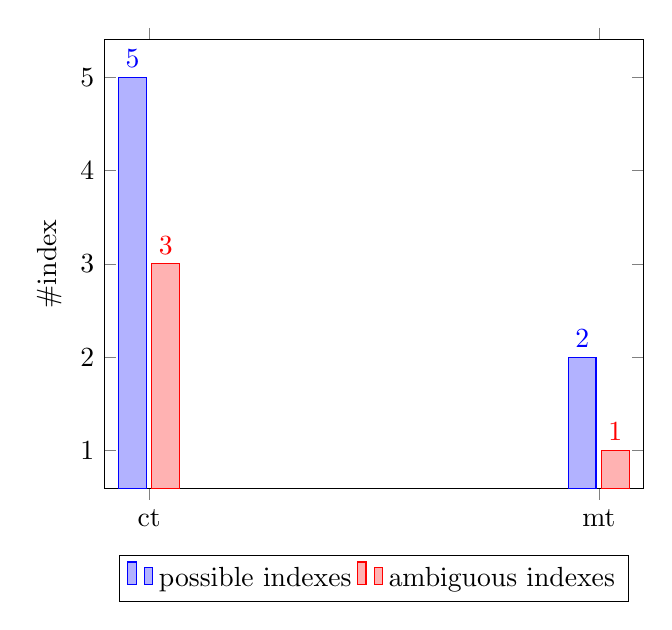
\begin{tikzpicture}
\begin{axis}[
    ybar,
    legend style={at={(0.5,-0.15)},
      anchor=north,legend columns=-1},
    symbolic x coords={ct,mt},
    ylabel={\#index},
    xtick=data,
    nodes near coords,
    nodes near coords align={vertical}
    ]
\addplot coordinates {(ct,5) (mt, 2)};
\addplot coordinates {(ct,3) (mt, 1)};
\legend{possible indexes, ambiguous indexes}
\end{axis}
\end{tikzpicture}
\caption[The index selections for MariaDB and query variant 1.]{The different
  indexes selected for MariaDB and the query variant 1, the possible index
  selections --- as in those considered by the query optimizer --- are shown next to
those actually selected.}\label{fig:plot:mariadb:query1}
\end{figure}